% Created 2016-11-10 Thu 19:36
\documentclass[a4paper, titlepage]{article}
\usepackage[mathletters]{ucs}
\usepackage[mathletters]{ucs}
\usepackage[utf8]{inputenc}
\usepackage[T1]{fontenc}
\usepackage{fixltx2e}
\usepackage{graphicx}
\usepackage{longtable}
\usepackage{float}
\usepackage{wrapfig}
\usepackage{rotating}
\usepackage[normalem]{ulem}
\usepackage{amsmath}
\usepackage{textcomp}
\usepackage{marvosym}
\usepackage{wasysym}
\usepackage{amssymb}
\usepackage{hyperref}
\tolerance=1000
\usepackage{minted}
\usepackage[margin=1in]{geometry}
\usepackage[polish]{babel}
\usepackage{fontspec}
\defaultfontfeatures{Ligatures=TeX}
\usepackage[small,sf,bf]{titlesec}
\setromanfont{Baskerville}
\setsansfont{Tahoma}
\setmonofont{Hack}
\author{Wojciech Polak, Klaudia Głocka, Rafał Ziembiński, Konrad Chojnecki}
\date{\today}
\title{Programowanie Zespołowe 2016}
\hypersetup{
  pdfkeywords={},
  pdfsubject={},
  pdfcreator={Emacs 25.1.1 (Org mode 8.2.10)}}
\begin{document}

\maketitle
\tableofcontents

\clearpage
\section{Opis aplikacji}
\label{sec-1}
Aplikacja ma za zadanie połączenie dwóch lub więcej urządzeń, poprzez protokół komunikacyjny \emph{Bluetooth}, w celu zapewnienia podstawowej komunikacji w postaci wiadomości tekstowych.
\subsection{Użyte technologie}
\label{sec-1-1}
Do stworzenia aplikacji użyto zestawu narzędzi firmy \emph{Xamarin}. Kod źródłowy aplikacji został napisany głównie w języku C\#.
Użyte biblioteki i oprogramowanie pozwoliło współdzielić kod dla wielu platform, tym samym umożliwiając szybki rozwój aplikacji zarówno na system \textbf{iOS} jak i \textbf{Android}.
\subsection{Zarys architektury aplikacji}
\label{sec-1-2}
Aplikacja została stworzona w oparciu o wzorzec projektowy \emph{Model - View - Controller}.

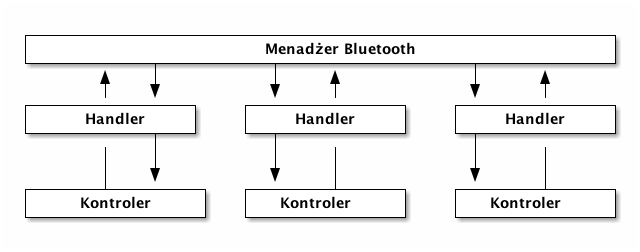
\includegraphics[width=.9\linewidth]{zarys.png}

\subsubsection{Moduł Menadżera Bluetooth}
\label{sec-1-2-1}
Menadżer Bluetooth odpowiada za najniższą warstwę aplikacji. Każdy z systemów - odpowiednio \textbf{iOS} jak i \textbf{Android} posiadają inne Programistyczne Interfejsy Aplikacji (w skrócie \emph{API}). Najniższa warstwa będąca \emph{najbliżej sprzętu} została rozdzielona pomiędzy systemy. Dlatego ten menadżer został zaimplementowany jako dwa moduły.

Ponieważ wymagane jest aby aplikacja w przyszłości była łatwo rozszerzalna, została wprowadzona warstwa abstrakcji - \texttt{IBluetoothManager} która służy jako punkt wyjścia i wejścia dla innych modułów.

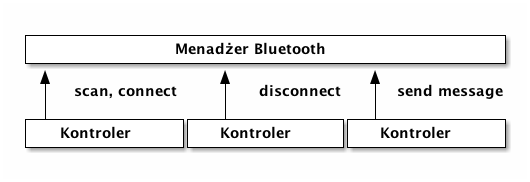
\includegraphics[width=.9\linewidth]{BM.png}

\subsubsection{Asynchroniczność aplikacji}
\label{sec-1-2-2}
Aplikacja jest zależna od zasobów zewnętrznych takich jak sieć \emph{Bluetooth}. W momencie gdy system czeka na nawiązanie połączenia z drugą komórką jest wymagane aby użytkownik cały czas miał aplikację interaktywną i responsywną. 

Aby aplikacja nie blokowała interfejsu użytkownika wszystkie akcje wykonywane przez warstwy niższe i pośrednie muszą być \textbf{asynchroniczne}.
Rozwiązaniem są moduły \texttt{Handlera} których zadaniem jest reakcja na wydarzenia.
\subsubsection{Moduł \texttt{Handler}}
\label{sec-1-2-3}
W momencie gdy zadanie zostanie wykonane (np. użytkownik zostanie połączony z innym), wiadomość zostaje wysłana do odpowiedniego \texttt{Handler} który reaguje w odpowiedni sposób do danych wejściowych.

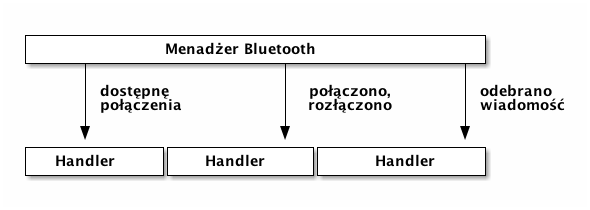
\includegraphics[width=.9\linewidth]{Handler.png}

W projekcie znajdują się dwa moduły typu \texttt{Handler}
\begin{enumerate}
\item Moduł \texttt{Message Handler}
\texttt{Message Handler} odpowiada za łączenie z innymi użytkownikami.
Do zadań tego modułu należą:
\begin{itemize}
\item Reakcja na pobraną listę dostępnych w pobliżu użytkowników - pseudonimy użytkowników są wyświetlane na ekranie.
\item Reakcja na połączenie się z danym użytkownikiem - następuje zmiana widoku na widok wysłanych i odebranych wiadomości.
\end{itemize}
\item Moduł \texttt{Connection Handler}
     \texttt{Connection Handler} odpowiada za reakcję na wiadomości odebrane od innego użytkownika. Wiadomości takie są wyświetlane w czytelnej formie na ekranie telefonu.
\end{enumerate}
\subsubsection{Modele}
\label{sec-1-2-4}

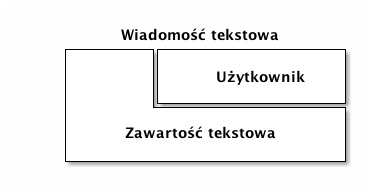
\includegraphics[width=.9\linewidth]{models.png}

\begin{enumerate}
\item Użytkownik
\label{sec-1-2-4-1}
Aplikacja przechowuje informacje o użytkowniku takie jak:
\begin{itemize}
\item pseudonim
\item unikalny identyfikator oparty o technologię \texttt{GUID4}
\end{itemize}
\item Wiadomość
\label{sec-1-2-4-2}
Wysyłane i odbierane wiadomości mają format:
\begin{itemize}
\item Użytkownik
\item Wiadomość tekstowa
\end{itemize}
\end{enumerate}
\subsubsection{Kontrolery}
\label{sec-1-2-5}
Kontrolery odpowiadają za zarządzanie danymi które zostały odebrane przez moduły \texttt{Handler}.
Często wymagane jest aby dane te zostały odpowiednio spreparowane zanim zostaną wyświetlone na ekranie.
Dobrą praktyką jest, aby w dalszych widokach \textbf{nie było żadnej logiki biznesowej}. Dlatego każda operacja na danych musi się odbyć w kontrolerze.

Kontrolery są modułami które odbierają wydarzenia (np. naciśnięcie przycisku, wpisanie tekstu, gesty czy ruch zarejestrowany przez akcelerator) które zostały wykonane w odpowiednich widokach.
Kontrolery reagują wydarzenia i na podstawie zawartości wydarzeń przesyłają odpowiednie komendy do pozostałych modułów, najczęściej do Menadżera Bluetooth.
\subsubsection{Widoki}
\label{sec-1-2-6}
Aplikacja składa się z dwóch widoków.
\begin{enumerate}
\item Widok z możliwymi połączeniami. 
W tym widoku użytkownik może zobaczyć wszystkich innych użytkowników, którzy są w zasięgu.
Urządzenie skanuje obszar w określonym interwale czasowym.
Użytkownik może nawiązać bezpośrednie połączenie z jednym użytkownikiem tym samym przechodzą do widoku drugiego.
\item Widok wymiany wiadomości.
W tym widoku użytkownik wysyła i odbiera wiadomości nadane przez drugiego użytkownika. Na raz możliwa jest rozmowa tylko z jednym użytkownikiem.
Użytkownik oprócz wysyłania wiadomości może także zakończyć rozmowę tym samym wracając do widoku pierwszego.
\end{enumerate}
\section{Podział prac}
\label{sec-2}
\subsection{Rafał Ziembiński - moduł \texttt{BluetoothManager} dla systemu Android}
\label{sec-2-1}
\subsection{Klaudia Głocka - moduł \texttt{ConnectionHandler}}
\label{sec-2-2}
\subsection{Konrad Chojnecki - moduł \texttt{MessageHandler}}
\label{sec-2-3}
\subsection{Wojciech Polak - moduł \texttt{BluetoothManager} dla systemu iOS}
\label{sec-2-4}
\section{Stan prac}
\label{sec-3}
\subsection{Na dzień 01-11-2016}
\label{sec-3-1}
\begin{enumerate}
\item Przerwa w pracy w wyniku dni wolnych od pracy
\item Poprawa dokumentu opisującego projekt. Wykorzystanie w tym celu \LaTeX{}.
\item Konfiguracja środowisk programistycznych:
\begin{itemize}
\item Próby instalacji IDE, wymaganych bibliotek i narzędzi pracy
\item Konfiguracja maszyn wirtualnych oraz urządzeń natywnych
\end{itemize}
\end{enumerate}
\subsection{Na dzień 10-11-2016}
\label{sec-3-2}
\begin{enumerate}
\item Reinstalacja systemu operacyjnego Microsoft Windows na jednym stanowisku pracy, konfiguracja wszystkich potrzebnych bibliotek, narzędzi i edytorów.
\item Usunięcie Visual Studio 2013 na drugim stanowisku pracy. Konfiguracja Visual Studio 2015.
\item Aktualizacja dokumentacji o grafy i wykresy połączeń pomiędzy modułami
\end{enumerate}
% Emacs 25.1.1 (Org mode 8.2.10)
\end{document}
